\section{Experimental Study}
\label{sec-exp}

\marked{We next present an extensive experimental study of our ensemble-enabled approach for link prediction.
Using real-life datasets, we conducted four sets of experiments to
evaluate: (1) the effectiveness and efficiency of our new bagging methods vs. bagging methods \cite{liang2016},
(2) the effectiveness and efficiency of our approach vs. conventional methods \Aa \cite{adamic} and \BIGCLAM \cite{yang-wsdm2013}, (3) the impacts of various factors and (4) the improvements of our new bagging methods.}

\eat{
We next present an extensive experimental study of our ensemble-enabled approach for link prediction.
Using real-life datasets, we conducted two sets of experiments to
evaluate: (1) the effectiveness and efficiency of our approach vs. conventional methods \Aa \cite{adamic} and \BIGCLAM \cite{yang-wsdm2013} and (2) the impacts of various factors.
}

\subsection{Experimental settings}

We first present our experimental settings.

\stitle{Datasets}. We used the following real-life network datasets,
which are from the Koblenz Network Collection \footnote{http://konect.uni-koblenz.de/}.

\noindent (1) \marked{ \Digg is a 5 year friendship graph of Digg users with
$279,630$ nodes and $1,731,653$ directed edges. }

\noindent (2) \YouTube is a 7 month  friendship network of YouTube users
with $3,223,589$ nodes and $9,375,374$ undirected edges.

\noindent (3) \Flickr is a 6 month friendship connections of Flickr users
with $2,302,925$ nodes and $33,140,017$ directed edges.

\noindent (4) \Wikipedia is a 6 year hyperlink network of the English Wikipedia
with $1,870,709$ nodes and $39,953,145$ directed edges.

\noindent (5) \Twitter is the follower network from Twitter with $41,652,230$ nodes
  and $1,468,365,182$ directed edges.

\noindent (6) \Friendster is the friendship network of the Friendster with $68,349,466$
  nodes and $2,586,147,869$ directed edges.



(1) \Digg, \YouTube, \Flickr and \Wikipedia contain timestamps of edge arrivals.
For each of these datasets, the latest five month part
is treated as its ground truth data for testing the accuracy, and the remaining part is treated as its training data,
shown in Table~\ref{tab_dataset}. To test the scalability, we further generated
five subnetworks with increasing sizes for each dataset, using the breadth first search started from the node
with the largest degree.
(2) \Twitter and \Friendster do not have
timestamps, and are only used for the scalability test.
(3) It does not make much sense to predict links for users
who appear in the ground truth data, but not in the training data. Hence, we removed these users from the ground truth data. Moreover, since our link prediction methods focus on predicting links on undirected graphs, we ignored the direction of edges in the directed graphs.




\begin{table}
\caption{Training and ground truth data. The data in the first time slot is the training data and
the remaining is the ground truth data.}
\label{tab_dataset}
\vspace{-2ex}
\centering
\begin{tabular}{cccc}
\hline \hline Datasets & Date & Nodes &  Edges  \\
\hline \hline
 & 2005-08-06 --- 2009-02-08 & 207,570 & 1,049,611 \\
\raisebox{1.0ex}[0pt]{ \Digg } & 2009-02-09 --- 2009-07-08 & 207,570 & 467,816 \\
\hline
 & 2006-12-09 --- 2007-02-22 & 1,503,841 & 3,691,893 \\
\raisebox{1.0ex}[0pt]{ \YouTube } & 2007-02-23 --- 2007-07-22 & 1,503,841 & 806,213 \\
\hline
  & 2006-11-01 --- 2006-11-30 & 1,580,291 & 13,341,698 \\
\raisebox{1.0ex}[0pt]{ \Flickr } & 2006-12-01 --- 2007-05-17 & 1,580,291 & 3,942,599 \\
\hline
 & 2001-02-19 --- 2006-10-31 & 1,682,759 & 28,100,011 \\
\raisebox{1.0ex}[0pt]{ \Wikipedia } & 2006-11-01 --- 2007-04-05 & 1,682,759 & 5,856,896\\
\hline \hline
\end{tabular}
\end{table}

\begin{table}
\caption{Parameters used in the experiments.
Note that we set $k = 1\times 10^5$ for \YouTube and $k =1\times 10^6$ for
other datasets.}
\label{tab_parameter}
\vspace{-2ex}
\centering
\newcommand{\tabincell}[2]{\begin{tabular}{@{}#1@{}}#2\end{tabular}}
\begin{tabular}{c l c}
\hline \hline Parameters & Descriptions & Default Values  \\
\hline \hline
 $\beta$  & Coefficient in \NMF update rule & 0.5\\
 $iter$   & Number of iterations for \NMF   & 50 \\
 $r$      & Number of latent factors       & 10  \\
\hline
$\epsilon$ & Tolerance of top-($\epsilon$, $k$) prediction & 1 \\
$k$        & \tabincell{l}{Number of links returned by \\ top-($\epsilon$, $k$) prediction} & $1\times 10^5 $ / $1\times 10^6$   \\
\hline
$\mu$ & \tabincell{l}{Expected appearing times of each \\
node pair in ensemble components} & 0.1 \\
$f$   & \tabincell{l}{Fraction of the number of nodes to be\\
 selected for an ensemble component} & 0.1 \\
$s$   & \marked{\tabincell{l}{Fraction of the number of edges to be\\
 selected for an ensemble component}} & 0.75 \\
\hline
$n$ & Number of nodes & See Table \ref{tab_dataset}\\
\hline \hline
\end{tabular}
\end{table}

\eat{ %%%%%%%%%%%%%%%%%%
\begin{figure*}[tb!]
  \centering
  %\vspace{-2ex}
  % Requires \usepackage{graphicx}
  \subfigure[YouTube]{\label{fig_exp1_k_acc_youtube}\includegraphics[width= 1.7in]{eps-script/1a.eps} }
  \quad\quad
  \subfigure[Flickr]{\label{fig_exp1_k_acc_flickr}\includegraphics[width= 1.7in]{eps-script/1b.eps}}
  \quad\quad
  \subfigure[Wikipedia]{\label{fig_exp1_k_acc_wikipedia}\includegraphics[width= 1.7in]{eps-script/1c.eps} }
  \quad\quad
  \subfigure[YouTube]{\label{fig_exp1_k_time_youtube}\includegraphics[width= 1.7in]{eps-script/1d.eps} }
  \quad\quad
  \subfigure[Flickr]{\label{fig_exp1_k_time_flickr}\includegraphics[width=  1.7in]{eps-script/1e.eps}}
  \quad\quad
  \subfigure[Wikipedia]{\label{fig_exp1_k_time_wikipedia}\includegraphics[width= 1.7in]{eps-script/1f.eps}}
  \vspace{-2ex}
  \caption{Accuracy and efficiency comparison: with respect to the number $k$ of predicted links.}\label{exp-k}
  \vspace{-2ex}
\end{figure*}

\begin{figure*}[tb!]
  \centering
  % Requires \usepackage{graphicx}
  \vspace{1ex}
  \subfigure[YouTube]{\label{fig_exp1_size_acc_youtube}\includegraphics[width= 1.7in]{eps-script/2a.eps}}
  \quad\quad
  \subfigure[Flickr]{\label{fig_exp1_size_acc_flickr}\includegraphics[width= 1.7in]{eps-script/2b.eps}}
  \quad\quad
  \subfigure[Wikipedia]{\label{fig_exp1_size_acc_wikipedia}\includegraphics[width= 1.7in]{eps-script/2c.eps}}
\quad\quad
\subfigure[YouTube]{\label{fig_exp1_size_time_youtube}\includegraphics[width= 1.7in]{eps-script/2d.eps}}
  \quad\quad
  \subfigure[Flickr]{\label{fig_exp1_size_time_flickr}\includegraphics[width= 1.7in]{eps-script/2e.eps}}
  \quad\quad
  \subfigure[Wikipedia]{\label{fig_exp1_size_time_wikipedia}\includegraphics[width= 1.7in]{eps-script/2f.eps}}
  \quad\quad
  \subfigure[Twitter]{\label{fig_exp1_size_time_twitter}\includegraphics[width= 1.7in]{eps-script/2g.eps}}
  \quad\quad
  \subfigure[Friendster]{\label{fig_exp1_size_time_friendster}\includegraphics[width= 1.7in]{eps-script/2h.eps}}
  \vspace{-2ex}
  \caption{Accuracy and efficiency comparison: with respect to the network sizes.}\label{exp-n}
  \vspace{-3ex}
\end{figure*}

} %%%%%%%%%%%%

\stitle{Algorithms for comparison}. We have carefully chosen a couple of algorithms
to compare with our ensemble-enabled approach.


  \noindent (1) \Adamic \cite{adamic}: \Aa is a popular neighborhood based method that
  produces a score for each link $(u, v)$, defined as below:
  \vspace{-2ex}
  \[ score(u, v) = \sum_{z \in N(u)\cap N(v)}\frac{1}{log|N(z)|}, \]
    \vspace{-.5ex}
  where $N(u)$ is the set of neighbors of node $u$. Lu \cite{linyuan-2011} showed that
  \Aa performs well on a range of networks because it only concerns 2-hop neighbors and
  reduces much of search space. Therefore, we implemented a top-$k$ link prediction
  method by searching the $k$ largest \Aa score links. The complexity of this method is
  $O(nd^2log(k))$, where $d$ is the average degree of networks. Another popular link
  prediction method is \Katz \cite{katz-1953}, which is based on the ensemble of all paths. However, its
  complexity is $O(n^3)$, and does not work on large networks with millions
  of nodes. Thus, we did not choose \Katz for comparison in the experiments.



  \noindent (2) \CAMBN \cite{yang-wsdm2013}:
  Yang and Leskovec developed this probabilistic generative model for networks
  based on community affiliations. An ingredient of \BIGCLAM is based on the fact that,
  when people share multiple community affiliations, the links between them stem for
  one dominant reason. This means that more communities a node pair shares,
  the higher the probability of the  node pair being connected is.
  Let $F$ be a nonnegative matrix where $F_{uc}$ is the degree of the node $u$ belongs to
  the community $c$. Give $F$, the \BIGCLAM generates a graph $G(N, A)$ by creating edge
  $(u, v)$ between a pair of nodes $u, v \in N$ with the probability
    \[ p(u, v) = 1 - exp(-F_u\cdot F_v), \]

\noindent  where $F_u$ is a weight vector for node $u$. Viewing the probability $p(u, v)$ as
  a score for the link $(u, v)$, it is reasonable to predict links based on \BIGCLAM.
The complexity of  \BIGCLAM is $O(nd(r + d) )$, where $d$ is the average degree of networks.
  In addition, this model is not designed to search the entire space of $O( n^2 )$,
  and we revised it by our top-($\epsilon$, $k$) method to predict links.


\stitle{Implementation}.
We implemented all algorithms including \Aa, \BIGCLAM, link prediction method in Section 2 (\NMF),
\NMF with random node bagging (\Node), \NMF with  edge bagging (\Edge) and
\NMF with biased edge bagging (\Biased), \marked{ \Nodep, \Edgep and \Biasedp} using C/C++ with no parallelization.


All experiments were conducted on a machine with 2 Intel Xeon
E5--2630 2.4GHz CPUs and 64 GB of Memory, running 64 bit
Windows 7 professional system. Each experiment was repeated 5 times,
and the average is reported here.



\subsection{Experimental Results}


We next present our findings. In all the experiments, we fixed $r$ to
$(50, 30, 50)$ (resp. $(40, 20, 20)$) for \NMF (resp. \BIGCLAM) on
\YouTube, \Flickr and \Wikipedia, respectively. For three bagging
methods, we fixed $r = 10$ by default (See Exp-2.3 for more details
about the setting of $r$). The other parameters with their
descriptions and default values are presented in Table \ref{tab_parameter}.





%%%%%%%%%%%%%%%%%%%%%%%%%%%%%%%%%%%%   2016-06-22 duan begin
\marked{\subsubsection{New Bagging vs. Bagging}
\stitle{Exp-1.1: Impacts of $k$}. The results of accuracy and running time are reported in Figure \ref{fig_exp_1_1}.  \\
\eat{\begin{table*}
\caption{Accuracy comparison: with respect to the number $k$ of predicted links.}
\label{tab_exp_1_1}
\vspace{-2ex}
\centering
\newcommand{\tabincell}[2]{\begin{tabular}{@{}#1@{}}#2\end{tabular}}
\begin{tabular}{l||c|c|c|c|c||c|c|c|c|c||c|c|c|c|c}
\hline \hline Dataset & \multicolumn{5}{c||}{YouTube}  & \multicolumn{5}{c||}{Flickr} & \multicolumn{5}{c}{Wikipedia}  \\
\hline
$k(\times 10^5) $  & 0.2 & 0.4 & 0.6 & 0.8 & 1 & 2 & 4 & 6 & 8 & 10 & 2 & 4 & 6 & 8 & 10 \\
\hline
\Node  & 3.65 & 2.87 & 2.60 & 2.43 & 2.26 & 11.06 & 9.46 & 8.70 & 8.17 & 7.56 & 4.09 & 3.09 & 2.69 & 2.49 & 2.26 \\
\Nodep  & 3.65 & 2.87 & 2.60 & 2.43 & 2.26 & 11.06 & 9.46 & 8.70 & 8.17 & 7.56 & 4.09 & 3.09 & 2.69 & 2.49 & 2.26 \\
\hline
\Edge & 3.77 & 2.94 & 2.66 & 2.48 & 2.30 & 11.01 & 9.49 & 8.73 & 8.20 & 7.61 & 4.03 & 3.14 & 2.71 & 2.51 & 2.27 \\
\Edgep & 3.77 & 2.94 & 2.66 & 2.48 & 2.30 & 11.01 & 9.49 & 8.73 & 8.20 & 7.61 & 4.03 & 3.14 & 2.71 & 2.51 & 2.27 \\
\hline
\Biased & 3.66 & 2.90 & 2.61 & 2.35 & 2.23 & 11.09 & 9.56 & 8.78 & 8.23 & 7.63 & 4.09 & 3.17 & 2.71 & 2.48 & 2.24 \\
\Biasedp & 3.64 & 2.82 & 2.60 & 2.36 & 2.24 & 11.14 & 9.50 & 8.72 & 8.16 & 7.56 & 4.01 & 3.17 & 2.73 & 2.49 & 2.24 \\
\hline \hline
\end{tabular}
\end{table*} } %%%%%%%%%%
\begin{figure*}[tb!]
  \centering
  %\vspace{-2ex}
  % Requires \usepackage{graphicx}
  \subfigure[Digg]{\label{fig_exp_1_1_k_acc_digg}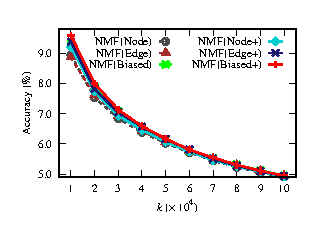
\includegraphics[width= 1.8in]{eps-script/1-1-a.eps} }
  \hspace{-3ex}
  \subfigure[YouTube]{\label{fig_exp_1_1_k_acc_youtube}\includegraphics[width= 1.8in]{eps-script/1-1-b.eps} }
  \hspace{-3ex}
  \subfigure[Flickr]{\label{fig_exp_1_1_k_acc_flickr}\includegraphics[width= 1.8in]{eps-script/1-1-c.eps}}
  \hspace{-3ex}
  \subfigure[Wikipedia]{\label{fig_exp_1_1_k_acc_wikipedia}\includegraphics[width= 1.8in]{eps-script/1-1-c.eps} }
  \subfigure[Digg]{\label{fig_exp_1_1_k_time_digg}\includegraphics[width= 1.8in]{eps-script/1-1-e.eps} }
  \hspace{-3ex}
  \subfigure[YouTube]{\label{fig_exp_1_1_k_time_youtube}\includegraphics[width= 1.8in]{eps-script/1-1-f.eps} }
  \hspace{-3ex}
  \subfigure[Flickr]{\label{fig_exp_1_1_k_time_flickr}\includegraphics[width=  1.8in]{eps-script/1-1-d.eps}}
  \hspace{-3ex}
  \subfigure[Wikipedia]{\label{fig_exp_1_1_k_time_wikipedia}\includegraphics[width= 1.8in]{eps-script/1-1-d.eps}}
  \vspace{-2ex}
  \caption{Accuracy and efficiency comparison: with respect to the number $k$ of predicted links.}\label{fig_exp_1_1}
  \vspace{-2ex}
\end{figure*}
\stitle{Exp-1.2: Impacts of network sizes}. The results of accuracy and running time are reported in Figure \ref{fig_exp_1_2}.\\
\begin{figure*}[tb!]
  \centering
  % Requires \usepackage{graphicx}
  \vspace{1ex}
  \subfigure[Digg]{\label{fig_exp_1_2_size_acc_digg}\includegraphics[width= 1.8in]{eps-script/1-2-a.eps}}
  \hspace{-3ex}
  \subfigure[YouTube]{\label{fig_exp_1_2_size_acc_youtube}\includegraphics[width= 1.8in]{eps-script/1-2-b.eps}}
  \hspace{-3ex}
  \subfigure[Flickr]{\label{fig_exp_1_2_size_acc_flickr}\includegraphics[width= 1.8in]{eps-script/1-2-c.eps}}
  \hspace{-3ex}
  \subfigure[Wikipedia]{\label{fig_exp_1_2_size_acc_wikipedia}\includegraphics[width= 1.8in]{eps-script/1-2-c.eps}}
  \subfigure[Digg]{\label{fig_exp_1_2_size_time_digg}\includegraphics[width= 1.8in]{eps-script/1-2-e.eps}}
  \hspace{-3ex}
  \subfigure[YouTube]{\label{fig_exp_1_2_size_time_youtube}\includegraphics[width= 1.8in]{eps-script/1-2-f.eps}}
  \hspace{-3ex}
  \subfigure[Flickr]{\label{fig_exp_1_2_size_time_flickr}\includegraphics[width= 1.8in]{eps-script/1-2-d.eps}}
  \hspace{-3ex}
  \subfigure[Wikipedia]{\label{fig_exp_1_2_size_time_wikipedia}\includegraphics[width= 1.8in]{eps-script/1-2-d.eps}}
  \subfigure[Twitter]{\label{fig_exp_1_2_size_time_twitter}\includegraphics[width= 1.8in]{eps-script/1-2-g.eps}}
  \quad\quad
  \subfigure[Friendster]{\label{fig_exp_1_2_size_time_friendster}\includegraphics[width= 1.8in]{eps-script/1-2-h.eps}}
  \vspace{-2ex}
  \caption{Accuracy and efficiency comparison: with respect to the network sizes.}\label{fig_exp_1_2}
  \vspace{-3ex}
\end{figure*}
\subsubsection{Comparison with \Aa and \BIGCLAM}
\stitle{Exp-2.1: Impacts of $k$}. The results of accuracy and running time are reported in Figure \ref{fig_exp_2_1}.\\
\begin{figure*}[tb!]
  \centering
  %\vspace{-2ex}
  % Requires \usepackage{graphicx}
  \subfigure[Digg]{\label{fig_exp_2_1_k_acc_digg}\includegraphics[width= 1.8in]{eps-script/2-1-a.eps} }
  \hspace{-3ex}
  \subfigure[YouTube]{\label{fig_exp_2_1_k_acc_youtube}\includegraphics[width= 1.8in]{eps-script/2-1-b.eps} }
  \hspace{-3ex}
  \subfigure[Flickr]{\label{fig_exp_2_1_k_acc_flickr}\includegraphics[width= 1.8in]{eps-script/2-1-c.eps}}
  \hspace{-3ex}
  \subfigure[Wikipedia]{\label{fig_exp_2_1_k_acc_wikipedia}\includegraphics[width= 1.8in]{eps-script/2-1-c.eps} }
  \subfigure[Digg]{\label{fig_exp_2_1_k_time_digg}\includegraphics[width= 1.8in]{eps-script/2-1-e.eps} }
  \hspace{-3ex}
  \subfigure[YouTube]{\label{fig_exp_2_1_k_time_youtube}\includegraphics[width= 1.8in]{eps-script/2-1-f.eps} }
  \hspace{-3ex}
  \subfigure[Flickr]{\label{fig_exp_2_1_k_time_flickr}\includegraphics[width=  1.8in]{eps-script/2-1-d.eps}}
  \hspace{-3ex}
  \subfigure[Wikipedia]{\label{fig_exp_2_1_k_time_wikipedia}\includegraphics[width= 1.8in]{eps-script/2-1-d.eps}}
  \vspace{-2ex}
  \caption{Accuracy and efficiency comparison: with respect to the number $k$ of predicted links.}\label{fig_exp_2_1}
  \vspace{-2ex}
\end{figure*}
\stitle{Exp-2.2: Impacts of network sizes}. The results of accuracy and running time are reported in Figure \ref{fig_exp_2_2}.\\
\begin{figure*}[tb!]
  \centering
  % Requires \usepackage{graphicx}
  \vspace{1ex}
  \subfigure[Digg]{\label{fig_exp_2_2_size_acc_digg}\includegraphics[width= 1.8in]{eps-script/2-2-a.eps}}
  \hspace{-3ex}
  \subfigure[YouTube]{\label{fig_exp_2_2_size_acc_youtube}\includegraphics[width= 1.8in]{eps-script/2-2-b.eps}}
  \hspace{-3ex}
  \subfigure[Flickr]{\label{fig_exp_2_2_size_acc_flickr}\includegraphics[width= 1.8in]{eps-script/2-2-c.eps}}
  \hspace{-3ex}
  \subfigure[Wikipedia]{\label{fig_exp_2_2_size_acc_wikipedia}\includegraphics[width= 1.8in]{eps-script/2-2-c.eps}}
  \subfigure[Digg]{\label{fig_exp_2_2_size_time_digg}\includegraphics[width= 1.8in]{eps-script/2-2-e.eps}}
  \hspace{-3ex}
  \subfigure[YouTube]{\label{fig_exp_2_2_size_time_youtube}\includegraphics[width= 1.8in]{eps-script/2-2-f.eps}}
  \hspace{-3ex}
  \subfigure[Flickr]{\label{fig_exp_2_2_size_time_flickr}\includegraphics[width= 1.8in]{eps-script/2-2-d.eps}}
  \hspace{-3ex}
  \subfigure[Wikipedia]{\label{fig_exp_2_2_size_time_wikipedia}\includegraphics[width= 1.8in]{eps-script/2-2-d.eps}}
  \hspace{-3ex}
  \subfigure[Twitter]{\label{fig_exp_2_2_size_time_twitter}\includegraphics[width= 1.8in]{eps-script/2-2-g.eps}}
  \quad\quad
  \subfigure[Friendster]{\label{fig_exp_2_2_size_time_friendster}\includegraphics[width= 1.8in]{eps-script/2-2-h.eps}}
  \vspace{-2ex}
  \caption{Accuracy and efficiency comparison: with respect to the network sizes.}\label{fig_exp_2_2}
  \vspace{-3ex}
\end{figure*}
\subsubsection{Impacts of Various Parameters}
\stitle{Exp-3.1: Impacts of $\mu$}. The results of accuracy and running time are reported in Figure \ref{fig_exp_3_mu}. \\
\begin{figure*}[tb!]
  \centering
  %\vspace{-2ex}
  % Requires \usepackage{graphicx}
  \subfigure[Digg]{\label{fig_exp_3_mu_acc_digg}\includegraphics[width= 1.8in]{eps-script/3-1-a.eps}}
  \hspace{-3ex}
  \subfigure[YouTube]{\label{fig_exp_3_mu_acc_youtube}\includegraphics[width= 1.8in]{eps-script/3-1-b.eps}}
  \hspace{-3ex}
  \subfigure[Flickr]{\label{fig_exp_3_mu_acc_flickr}\includegraphics[width=1.8in]{eps-script/3-1-c.eps}}
  \hspace{-3ex}
  \subfigure[Wikipedia]{\label{fig_exp_3_mu_acc_wikipedia}\includegraphics[width=1.8in]{eps-script/3-1-c.eps}}
  \subfigure[Digg]{\label{fig_exp_3_mu_time_digg}\includegraphics[width=1.8in]{eps-script/3-1-e.eps}}
  \hspace{-3ex}
  \subfigure[YouTube]{\label{fig_exp_3_mu_time_youtube}\includegraphics[width=1.8in]{eps-script/3-1-f.eps}}
  \hspace{-3ex}
  \subfigure[Flickr]{\label{fig_exp_3_mu_time_flickr}\includegraphics[width=1.8in]{eps-script/3-1-d.eps}}
  \hspace{-3ex}
  \subfigure[Wikipedia]{\label{fig_exp_3_mu_time_wikipedia}\includegraphics[width=1.8in]{eps-script/3-1-d.eps}}
  \vspace{-2ex}
  \caption{Accuracy and efficiency comparison: with respect to the expected appearing times $\mu$.}\label{fig_exp_3_mu}
  \vspace{-2ex}
\end{figure*}
\stitle{Exp-3.2: Impacts of $f$}. The results of accuracy and running time are reported in Figure. \\
\begin{figure*}[tb!]
  \centering
  \vspace{1ex}
  % Requires \usepackage{graphicx}
  \subfigure[Digg]{\label{fig_exp_3_f_acc_digg}\includegraphics[width= 1.8in]{eps-script/3-2-a.eps} }
  \hspace{-3ex}
  \subfigure[YouTube]{\label{fig_exp_3_f_acc_youtube}\includegraphics[width= 1.8in]{eps-script/3-2-b.eps} }
  \hspace{-3ex}
  \subfigure[Flickr]{\label{fig_exp_3_f_acc_flickr}\includegraphics[width= 1.8in]{eps-script/3-2-c.eps} }
  \hspace{-3ex}
  \subfigure[Wikipedia]{\label{fig_exp_3_f_acc_wikipedia}\includegraphics[width= 1.8in]{eps-script/3-2-c.eps} }
  \subfigure[Digg]{\label{fig_exp_3_f_time_digg}\includegraphics[width= 1.8in]{eps-script/3-2-e.eps} }
  \hspace{-3ex}
  \subfigure[YouTube]{\label{fig_exp_3_f_time_youtube}\includegraphics[width= 1.8in]{eps-script/3-2-f.eps} }
  \hspace{-3ex}
  \subfigure[Flickr]{\label{fig_exp_3_f_time_flickr}\includegraphics[width= 1.8in]{eps-script/3-2-d.eps}}
  \hspace{-3ex}
  \subfigure[Wikipedia]{\label{fig_exp_3_f_time_wikipedia}\includegraphics[width= 1.8in]{eps-script/3-2-d.eps}}
  \vspace{-2ex}
  \caption{Accuracy and efficiency comparison: with respect to the fraction $f$}\label{fig_exp_3_f}
  \vspace{-3ex}
\end{figure*}
\stitle{Exp-3.3: Impacts of $s$}. The results of accuracy and running time are reported in Figure \ref{fig_exp_3_s}. \\
\begin{figure*}[tb!]
  \centering
  \vspace{1ex}
  % Requires \usepackage{graphicx}
  \subfigure[Digg]{\label{fig_exp_3_s_acc_digg}\includegraphics[width= 1.8in]{eps-script/3-3-a.eps} }
  \hspace{-3ex}
  \subfigure[YouTube]{\label{fig_exp_3_s_acc_youtube}\includegraphics[width= 1.8in]{eps-script/3-3-b.eps} }
  \hspace{-3ex}
  \subfigure[Flickr]{\label{fig_exp_3_s_acc_flickr}\includegraphics[width= 1.8in]{eps-script/3-3-c.eps} }
  \hspace{-3ex}
  \subfigure[Wikipedia]{\label{fig_exp_3_s_acc_wikipedia}\includegraphics[width= 1.8in]{eps-script/3-3-c.eps} }
  \subfigure[Digg]{\label{fig_exp_3_s_time_digg}\includegraphics[width= 1.8in]{eps-script/3-3-e.eps} }
  \hspace{-3ex}
  \subfigure[YouTube]{\label{fig_exp_3_s_time_youtube}\includegraphics[width= 1.8in]{eps-script/3-3-f.eps} }
  \hspace{-3ex}
  \subfigure[Flickr]{\label{fig_exp_3_s_time_flickr}\includegraphics[width= 1.8in]{eps-script/3-3-d.eps}}
  \hspace{-3ex}
  \subfigure[Wikipedia]{\label{fig_exp_3_s_time_wikipedia}\includegraphics[width= 1.8in]{eps-script/3-3-d.eps}}
  \vspace{-2ex}
  \caption{Accuracy and efficiency comparison: with respect to the fraction $s$}\label{fig_exp_3_s}
  \vspace{-3ex}
\end{figure*}
\stitle{Exp-3.4: Impacts of $r$}. The results of accuracy and running time are reported in Figure \ref{fig_exp_3_r}. \\
\begin{figure*}[tb!]
  \centering
  \vspace{1ex}
  % Requires \usepackage{graphicx}
  \subfigure[Digg]{\label{fig_exp_3_r_acc_digg}\includegraphics[width= 1.8in]{eps-script/3-4-a.eps} }
  \hspace{-3ex}
  \subfigure[YouTube]{\label{fig_exp_3_r_acc_youtube}\includegraphics[width= 1.8in]{eps-script/3-4-b.eps} }
  \hspace{-3ex}
  \subfigure[Flickr]{\label{fig_exp_3_r_acc_flickr}\includegraphics[width= 1.8in]{eps-script/3-4-c.eps} }
  \hspace{-3ex}
  \subfigure[Wikipedia]{\label{fig_exp_3_r_acc_wikipedia}\includegraphics[width= 1.8in]{eps-script/3-4-c.eps} }
  \subfigure[Digg]{\label{fig_exp_3_r_time_digg}\includegraphics[width= 1.8in]{eps-script/3-4-e.eps} }
  \hspace{-3ex}
  \subfigure[YouTube]{\label{fig_exp_3_r_time_youtube}\includegraphics[width= 1.8in]{eps-script/3-4-f.eps} }
  \hspace{-3ex}
  \subfigure[Flickr]{\label{fig_exp_3_r_time_flickr}\includegraphics[width= 1.8in]{eps-script/3-4-d.eps}}
  \hspace{-3ex}
  \subfigure[Wikipedia]{\label{fig_exp_3_r_time_wikipedia}\includegraphics[width= 1.8in]{eps-script/3-4-d.eps}}
  \vspace{-2ex}
  \caption{Accuracy and efficiency comparison: with respect to the fraction $f$}\label{fig_exp_3_r}
  \vspace{-3ex}
\end{figure*}
\stitle{Exp-3.5: Impacts of $\epsilon$}. The results of accuracy and running time are reported in Figure \ref{fig_exp_3_e}. \\
\begin{figure*}[tb!]
  \centering
  \vspace{1ex}
  % Requires \usepackage{graphicx}
  \subfigure[Digg]{\label{fig_exp_3_e_acc_digg}\includegraphics[width= 1.8in]{eps-script/3-5-a.eps} }
  \hspace{-3ex}
  \subfigure[YouTube]{\label{fig_exp_3_e_acc_youtube}\includegraphics[width= 1.8in]{eps-script/3-5-b.eps} }
  \hspace{-3ex}
  \subfigure[Flickr]{\label{fig_exp_3_e_acc_flickr}\includegraphics[width= 1.8in]{eps-script/3-5-c.eps} }
  \hspace{-3ex}
  \subfigure[Wikipedia]{\label{fig_exp_3_e_acc_wikipedia}\includegraphics[width= 1.8in]{eps-script/3-5-c.eps} }
  \subfigure[Digg]{\label{fig_exp_3_e_time_digg}\includegraphics[width= 1.8in]{eps-script/3-5-e.eps} }
  \hspace{-3ex}
  \subfigure[YouTube]{\label{fig_exp_3_e_time_youtube}\includegraphics[width= 1.8in]{eps-script/3-5-f.eps} }
  \hspace{-3ex}
  \subfigure[Flickr]{\label{fig_exp_3_e_time_flickr}\includegraphics[width= 1.8in]{eps-script/3-5-d.eps}}
  \hspace{-3ex}
  \subfigure[Wikipedia]{\label{fig_exp_3_e_time_wikipedia}\includegraphics[width= 1.8in]{eps-script/3-5-d.eps}}
  \vspace{-2ex}
  \caption{Accuracy and efficiency comparison: with respect to the fraction $f$}\label{fig_exp_3_e}
  \vspace{-3ex}
\end{figure*}
\subsubsection{Improvements}
\stitle{Exp-4: Improvements of new methods}. The results of running time are reported in Table \ref{tab_improvements}. \\
\begin{table}
\caption{Running time of different methods.}
\label{tab_improvements}
\vspace{-2ex}
\centering
\newcommand{\tabincell}[2]{\begin{tabular}{@{}#1@{}}#2\end{tabular}}
\begin{tabular}{l|c|c|c|c}
\hline \hline Methods & Digg & YouTube & Wikipedia & Flickr \\
\hline \hline
node + top-k            & 66    & 42.72 & 255.30 & 127.08 \\
node + new top-k        & 63    & 40.12 & 250.32 & 125.36 \\
new node + top-k        & 62    & 39.12 & 248.36 & 124.39 \\
new node + new top-k    & 59    & 38.12 & 244.12 & 121.03 \\
\hline
edge + top-k            & 75    & 47.30 & 289.83 & 129.06 \\
edge + new top-k        & 74    & 45.12 & 282.12 & 127.32 \\
new edge + top-k        & 73    & 43.12 & 275.12 & 124.32 \\
new edge + new top-k    & 72    & 42.12 & 265.12 & 119.32 \\
\hline
biased + top-k          & 56    & 42.89 & 204.84 & 117.32 \\
biased + new top-k      & 54    & 40.12 & 198.36 & 115.32 \\
new biased + top-k      & 52    & 38.12 & 195.69 & 112.32 \\
new biased + new top-k  & 50    & 36.12 & 189.35 & 110.32 \\
\hline \hline
\end{tabular}
\end{table}
\subsubsection{Limitations}
In this set of tests, we analysis the limitations of our ensemble enabled methods compared with \NMF.
}

%%%%%%%%%%%%%%%%%%%%%%%%%%%%%%%%%%%%   2016-06-22 duan end

\subsubsection{Comparison with \Aa and \BIGCLAM }



In the first set of tests,
we evaluated the effectiveness and efficiency of our methods compared with \Aa and
\BIGCLAM. Given one of top-$k$ link prediction methods, denoted by $x$, its effectiveness
of link prediction is evaluated with the following measure:
\begin{equation}
accuracy(x) = \frac{\# \textrm{ of correctly predicted links}}{\textrm{the number} \ k\ \textrm{of predicted links}}.
\end{equation}

%\[ accuracy(x) = \frac{\# \text{ of correctly predicted links}}{\text{the number}\ k\ \text{of predicted links}}. \]



\stitle{Exp-1.1: Impacts of $k$}. To evaluate the impacts of the number $k$ of predicted links, we varied $k$
from $1\times 10^4$ to $1\times 10^5$ on \YouTube (resp. from $1\times 10^5$ to $1\times 10^6$ on
\Flickr and \Wikipedia) and fixed other parameters to their default values.
The results of accuracy and running time are reported in Figure \ref{fig_exp1_k_acc_youtube},
\ref{fig_exp1_k_acc_flickr} and \ref{fig_exp1_k_acc_wikipedia} and Figure \ref{fig_exp1_k_time_youtube},
\ref{fig_exp1_k_time_flickr} and \ref{fig_exp1_k_time_wikipedia}, respectively.




The accuracy results tell us that (a) \Biased
outperforms other methods on all datasets, (b) three bagging methods always have higher accuracy than \NMF, \Aa
and \BIGCLAM,  (c) \NMF is more accurate
than \Aa and \BIGCLAM, and (d) the accuracy of all methods decreases with the increment of $k$.
Indeed, \Biased improves the accuracy by $(18\%, 39\%, 33\%)$ (resp. $(4\%, 10\%, 18\%)$
and $(16\%, 11\%, 38\%)$ ) over \NMF, \Aa and \BIGCLAM on \YouTube, \Flickr and \Wikipedia,
respectively. This verifies the effectiveness of our bagging methods.


The running time results tell us that (a) three
bagging methods are much faster than \NMF, \Aa and \BIGCLAM, (b) the running time of
all methods is insensitive to the increase of $k$, except \Aa whose complexity is
$O(nd^2log(k))$. Indeed, the three bagging methods finished the prediction in 300 seconds on the
three datasets. Furthermore, \Biased is $(70, 2.7, 14)$ (resp. $(4.5, 2.7, 8)$ and $(33, 33, 36)$) times faster than \NMF, \Aa and
\BIGCLAM on \YouTube, \Flickr and \Wikipedia, respectively. This verifies the
efficiency of our bagging methods.


Note that the accuracy of all methods is not high, even the best
accuracy (\Biased on \Flickr when $k = 1\times 10^5$) is less than $12\%$. The reason is that
there are more than $1\times 10^{12}$ possible links in the search space of each dataset,
but less than $1\times 10^7$ links in the ground truth.
In addition, \NMF is slower than \Aa on three datasets because $r$ is fixed to at least $30$, which is consistent to the
$O(nr^2)$ complexity of \NMF. The running time
of \Aa is about 100 seconds on \YouTube,
while more than 500 seconds on \Flickr and 4700 seconds on \Wikipedia. This is because that the average degree of these datasets are 5, 17 and 33, and \Aa takes more time with the increase of the degree of networks.
The running time of \BIGCLAM is also sensitive to the degree of networks because its complexity is $O(nd(r + d))$.
As a result, it runs faster than
\NMF on \YouTube when the degree is 5, while it takes more time on \Flickr and \Wikipedia
when the degree is increased.






\stitle{Exp-1.2: Impacts of network sizes}. To evaluate the impacts of network sizes, we varied the
number of nodes $n$ from $3\times 10^5$ to $1.5\times 10^6$ on \YouTube, \Flickr and \Wikipedia (resp.
from $3\times 10^5$ to $5\times 10^6$ on \Twitter and from $1\times 10^6$ to $1.5\times 10^7$ on
\Friendster). Since \Twitter and \Friendster do not contain
ground truth for choosing the value of $r$, we fixed $r$ on these datasets to the average value of
its default values. Hence, on these two datasets, we fixed $r = 43$ for \NMF
(resp. $r = 27$ for \BIGCLAM and $r = 10$ for bagging methods).
The other parameters are fixed to their default values.
The results of accuracy and running time are reported in Figure \ref{fig_exp1_size_acc_youtube},
\ref{fig_exp1_size_acc_flickr} and \ref{fig_exp1_size_acc_wikipedia} and Figure \ref{fig_exp1_size_time_youtube},
\ref{fig_exp1_size_time_flickr}, \ref{fig_exp1_size_time_wikipedia}, \ref{fig_exp1_size_time_twitter} and
\ref{fig_exp1_size_time_friendster}, respectively. Note that there are {\em some missing plots} for \NMF, \Aa and
\BIGCLAM in the Figure \ref{fig_exp1_size_time_twitter} and
\ref{fig_exp1_size_time_friendster} because their running time
is beyond 24 hours.



The accuracy results tell us that (a) \Biased obtains the highest accuracy on all
datasets, (b) the three bagging methods perform better than \NMF, \Aa and \BIGCLAM,
and (c) \NMF has higher accuracy than \Aa and \BIGCLAM. This means that
our methods are accurate and robust with the increase of network sizes.

The running time results tell us that (a) bagging methods are much faster than other methods,
(b) the running time of all methods increase nearly linearly with the increase of $n$. For
instance, \Biased speeds up \NMF, \Aa and \BIGCLAM for around $(20, 107, 43)$ (resp. $(31, 21, 175)$)
times on \Twitter (resp. \Friendster) and is thus essential for
making our bagging methods scalable to large networks. Note
that \NMF is slower than \BIGCLAM on \YouTube but faster on other datasets
because \BIGCLAM requires more time with the increase of the degree of networks,
which is consistent with the complexity analysis.
In addition, the running time of \BIGCLAM fluctuates when
$n$ between $6\times 10^5$ and $1.2\times 10^6$ on \YouTube and \Flickr because the number of
the iterations for its nonnegative matrix factorization method is not fixed.


\eat{ %%%%%%%%%%%
\begin{figure*}[tb!]
  \centering
  %\vspace{-2ex}
  % Requires \usepackage{graphicx}
  \subfigure[YouTube]{\label{fig_exp2_mu_acc_youtube}\includegraphics[width= 1.7in]{eps-script/3a.eps}}
  \quad\quad
  \subfigure[Flickr]{\label{fig_exp2_mu_acc_flickr}\includegraphics[width=1.7in]{eps-script/3b.eps}}
  \quad\quad
  \subfigure[Wikipedia]{\label{fig_exp2_mu_acc_wikipedia}\includegraphics[width=1.7in]{eps-script/3c.eps}}
\quad\quad
\subfigure[YouTube]{\label{fig_exp2_mu_time_youtube}\includegraphics[width=1.7in]{eps-script/3d.eps}}
  \quad\quad
  \subfigure[Flickr]{\label{fig_exp2_mu_time_flickr}\includegraphics[width=1.7in]{eps-script/3e.eps}}
  \quad\quad
  \subfigure[Wikipedia]{\label{fig_exp2_mu_time_wikipedia}\includegraphics[width=1.7in]{eps-script/3f.eps}}
  \vspace{-2ex}
  \caption{Accuracy and efficiency comparison: with respect to the expected appearing times $\mu$.}\label{fig_exp2_mu}
  \vspace{-2ex}
\end{figure*}
\begin{figure*}[tb!]
  \centering
  \vspace{1ex}
  % Requires \usepackage{graphicx}
  \subfigure[YouTube]{\label{fig_exp2_f_acc_youtube}\includegraphics[width= 1.7in]{eps-script/4a.eps} }
  \quad\quad
  \subfigure[Flickr]{\label{fig_exp2_f_acc_flickr}\includegraphics[width= 1.7in]{eps-script/4b.eps} }
  \quad\quad
  \subfigure[Wikipedia]{\label{fig_exp2_f_acc_wikipedia}\includegraphics[width= 1.7in]{eps-script/4c.eps} }
\quad\quad
  \subfigure[YouTube]{\label{fig_exp2_f_time_youtube}\includegraphics[width= 1.7in]{eps-script/4d.eps} }
  \quad\quad
  \subfigure[Flickr]{\label{fig_exp2_f_time_flickr}\includegraphics[width= 1.7in]{eps-script/4e.eps}}
  \quad\quad
  \subfigure[Wikipedia]{\label{fig_exp2_f_time_wikipedia}\includegraphics[width= 1.7in]{eps-script/4f.eps}}
  \vspace{-2ex}
  \caption{Accuracy and efficiency comparison: with respect to the fraction $f$}\label{fig_exp2_f}
  \vspace{-3ex}
\end{figure*}
}%%%%%%%%%%%%%%%%%%






\subsubsection{Impacts of Various Parameters}
In the second set of tests, we evaluated the impacts of parameters on
the accuracy and running time of \NMF, \Node, \Edge, \Biased and \BIGCLAM. We first
tested the impacts of $\mu$ and $f$ in bagging methods. We then
tested the impacts of $r$ and $\epsilon$.



\stitle{Exp-2.1: Impacts of $\mu$}. To evaluate the impacts of $\mu$, we
varied $\mu$ from $0.01$ to $0.25$ and fixed other parameters to their
default values. The accuracy and running time results are reported in
Figure \ref{fig_exp2_mu_acc_youtube}, \ref{fig_exp2_mu_acc_flickr} and
\ref{fig_exp2_mu_acc_wikipedia} and Figure \ref{fig_exp2_mu_time_youtube},
\ref{fig_exp2_mu_time_flickr} and \ref{fig_exp2_mu_time_wikipedia},
respectively. We also plotted the accuracy and running time of \NMF for comparison.




The results tell us that (a) bagging methods have higher accuracy than
\NMF when $\mu$ is large enough, (b) the accuracy of bagging methods
increases with the increment of $\mu$ and becomes stable when $\mu$ is greater
than $0.1$. This means that the accuracy of bagging methods would increase and become stable with
the increase of the number of ensemble components. Furthermore,
(c) the running time of bagging methods increases linearly
with the increase of $\mu$ since $\mu / f^2$ ensemble components had been generated in each bagging
method. Note that, when $\mu = 0.1$, the accuracy of bagging methods
is becoming stable and the running time of them is less than
\NMF. Therefore, we fixed $\mu = 0.1$ by default.




\stitle{Exp-2.2: Impacts of $f$}. To evaluate the impacts of $f$, we
varied $f$ from $0.02$ to $0.5$ and fixed other parameters to their
default values. The accuracy and running time results are reported in
Figure \ref{fig_exp2_f_acc_youtube}, \ref{fig_exp2_f_acc_flickr} and
\ref{fig_exp2_f_acc_wikipedia} and Figure \ref{fig_exp2_f_time_youtube},
\ref{fig_exp2_f_time_flickr} and \ref{fig_exp2_f_time_wikipedia}, respectively.



The results tell us that (a) bagging methods have higher accuracy
than \NMF when $f$ between 0.02 and 0.1, (b) the accuracy of bagging methods decreases
with the increase of $f$, and (c) the running time of bagging methods increases
nearly linearly with the decrease of $f$. Note that the complexity of bagging methods is
$O((n_{1}r^2 + n_{1}d_{1}r)*\mu /f^2)$, where $n_1 = nf$ and $d_1$ is the average degree of
each ensemble component. Since bagging methods are likely to select dense components, $d_1$
may be greater than $r$ and the complexity is $O(nd_1r\mu /f)$. Thus, the running time
of bagging methods increases with the decrease of $f$. Keeping the accuracy of bagging
methods better than that of \NMF, we fixed $f = 0.1$ by default to achieve a better efficiency.

\eat{%%%%%%%%%%%%%%
\begin{figure*}[tb!]
  \centering
  %\vspace{2ex}
  % Requires \usepackage{graphicx}
  \subfigure[YouTube]{\label{fig_exp2_r_acc_youtube}\includegraphics[width= 1.7in]{eps-script/5a.eps}}
  \quad\quad
  \subfigure[Flickr]{\label{fig_exp2_r_acc_flickr}\includegraphics[width= 1.7in]{eps-script/5b.eps}}
  \quad\quad
  \subfigure[Wikipedia]{\label{fig_exp2_r_acc_wikipedia}\includegraphics[width= 1.7in]{eps-script/5c.eps}}
\quad\quad
  \subfigure[YouTube]{\label{fig_exp2_r_time_youtube}\includegraphics[width= 1.7in]{eps-script/5d.eps}}
  \quad\quad
  \subfigure[Flickr]{\label{fig_exp2_r_time_flickr}\includegraphics[width= 1.7in]{eps-script/5e.eps}}
  \quad\quad
  \subfigure[Wikipedia]{\label{fig_exp2_r_time_wikipedia}\includegraphics[width= 1.7in]{eps-script/5f.eps}}
  \vspace{-2ex}
  \caption{Accuracy and efficiency comparison: with respect to the number $r$ of latent factors.}\label{fig_exp2_r}
  \vspace{-2ex}
\end{figure*}
\begin{figure*}[tb!]
  \centering
  \vspace{1ex}
  % Requires \usepackage{graphicx}
  \subfigure[YouTube]{\label{fig_exp2_e_acc_youtube}\includegraphics[width= 1.7in]{eps-script/6a.eps} }
  \quad\quad
  \subfigure[Flickr]{\label{fig_exp2_e_acc_flickr}\includegraphics[width= 1.7in]{eps-script/6b.eps}}
  \quad\quad
  \subfigure[Wikipedia]{\label{fig_exp2_e_acc_wikipedia}\includegraphics[width= 1.7in]{eps-script/6c.eps}}
  \quad\quad
  \subfigure[YouTube]{\label{fig_exp2_e_time_youtube}\includegraphics[width= 1.7in]{eps-script/6d.eps}}
  \quad\quad
  \subfigure[Flickr]{\label{fig_exp2_e_time_flickr}\includegraphics[width= 1.7in]{eps-script/6e.eps}}
  \quad\quad
  \subfigure[Wikipedia]{\label{fig_exp2_e_time_wikipedia}\includegraphics[width= 1.7in]{eps-script/6f.eps}}
  \vspace{-2ex}
  \caption{Accuracy and efficiency comparison: with respect to the tolerance $\epsilon$
  of top-($\epsilon, k$) prediction. }\label{fig_exp2_e}
  \vspace{-3ex}
\end{figure*}
} %%%%%%%%%%%%%%%%%


\stitle{Exp-2.3: Impacts of $r$}. To evaluate the impacts of $r$, we
varied $r$ from $10$ to $50$ and fixed other parameters to their
default values. The accuracy and running time results are reported in
Figure \ref{fig_exp2_r_acc_youtube}, \ref{fig_exp2_r_acc_flickr} and
\ref{fig_exp2_r_acc_wikipedia} and Figure \ref{fig_exp2_r_time_youtube},
\ref{fig_exp2_r_time_flickr} and \ref{fig_exp2_r_time_wikipedia}, respectively.



The results tell us that (a) \Biased obtains the best accuracy compared with other
methods, (b) bagging methods have higher accuracy than \NMF and \BIGCLAM,
(c) the accuracy of \NMF increases slightly with the increase of $r$ and is always
greater than that of \BIGCLAM, and (d) the running time of \NMF is increased
quadratically with the increase of $r$ since its complexity is $O(nr^2)$.
A similar trend of running time is also found for bagging methods. To obtain the
highest accuracy, we fixed $r$ to $(50, 30, 50)$ (resp. $(40, 20, 20)$) for \NMF
(resp. \BIGCLAM) on \YouTube, \Flickr and \Wikipedia, respectively. Note that, when $r = 10$,
the accuracy of bagging methods is greater than the best accuracy of \NMF. Hence, we
fixed $r = 10$ by default for bagging methods.

%Observe that
%\BIGCLAM performs worse on \Flickr and \Wikipedia when $r > 20$.
%This might be caused by its initialization process.



\stitle{Exp-2.4: Impacts of $\epsilon$}. To evaluate the impacts of $\epsilon$, we
varied $\epsilon$ from $0.5$ to $1.0$ and fixed other parameters to their
default values. The accuracy and running time results are reported in
Figure \ref{fig_exp2_e_acc_youtube}, \ref{fig_exp2_e_acc_flickr} and
\ref{fig_exp2_e_acc_wikipedia} and Figure \ref{fig_exp2_e_time_youtube},
\ref{fig_exp2_e_time_flickr} and \ref{fig_exp2_e_time_wikipedia}, respectively.



The results tell us that (a) the accuracy of all methods is stable with
the increase of $\epsilon$, which means that the accuracy of our methods is insensitive
to $\epsilon$, and (b) the running time of all methods is decreased with the increase of $\epsilon$
because the larger $\epsilon$ reduces more search space. Thus, our top-($\epsilon$, $k$)
method is reasonable for link prediction. Since the accuracy is insensitive to $\epsilon$, we
fixed $\epsilon = 1$ by default to achieve a better efficiency.






\stitle{Summary}. From these experimental results on real-life social network datasets,
we find the following. (1) \NMF is able to predict links and can be sped up
by the top-($\epsilon$, $k$) process to explore the $O(n^2)$ search space. It is
more accurate than \Aa and \BIGCLAM, which verifies the effectiveness
of \NMF. Moreover, \NMF runs faster than \BIGCLAM on dense networks,
e.g., \Flickr and \Wikipedia, which is consistent with the complexity analysis
that \BIGCLAM is sensitive to the degree of networks. (2) However, the running time of
\NMF is increased quadratically with the increase of $r$. This might be a bottleneck
for large networks. By decomposing the link prediction problem into smaller pieces
and solving them independently, our bagging methods are more efficient and
scale well with the size and density of large networks,
e.g., \Biased finished in an hour on \Friendster with $1.5\times 10^7$ nodes and
$1.0\times 10^9$ edges, while \NMF, \Aa  and \BIGCLAM could not finish in a day. Further, \Biased speeds up \NMF, \Aa and \BIGCLAM
for around $(20, 107, 43)$ (resp. $(31, 21, 175)$) times on \Twitter (resp. \Friendster).
(3) Combining link prediction characteristics, our
bagging methods also provide the accuracy advantages for link prediction,
e.g., \Biased is faster than the other methods, and improves the accuracy by
$(18\%, 39\%, 33\%)$ (resp. $(4\%, 10\%, 18\%)$ and $(16\%, 11\%, 38\%)$ )
over \NMF, \Aa and \BIGCLAM on \YouTube, \Flickr and \Wikipedia,
respectively.






%
%There are quite a few things that we can show here:
%
%\stitle{Exp-1: Efficiency tests}. We need to show how well our approach
%scales with increasing network size, and the fact that the approach
%remains practically feasible over a much broader range of network
%sizes. So we need some really large real networks, and then by using
%subsets of this network, we can show scalability with increasing
%network size.  A key question here is the choice of baseline to use.
%There are quite a few relevant works belonging to Nitesh Chawla. One
%baseline can of course be our own matrix factorization method
%without the ensembling. But we also need some external and state of
%the art baselines.
%
%
%
%
%\stitle{Exp-2: Accuracy tests}. Ensemble-based methods have the reputation of also
%improving the  accuracy. So it may make sense to check how well the
%approach performs against (i)  the matrix factorization approach
%without ensembling (ii) external baselines.


